\documentclass[11pt]{article}
\usepackage[utf8]{inputenc}
\setlength{\parindent}{1em}
\setlength{\parskip}{1em}
\usepackage{apacite}
\usepackage{graphicx}
\usepackage{float}
\usepackage{listings}
\usepackage{amsmath}
\usepackage{geometry}
\usepackage{algorithm}
\geometry{margin=4cm}
\begin{document}
\title{
  Matlab prosjekt}
\author{\small Roshan Azam\\ IN3190}
\maketitle

Oppgave 1)

\begin{figure}[H]
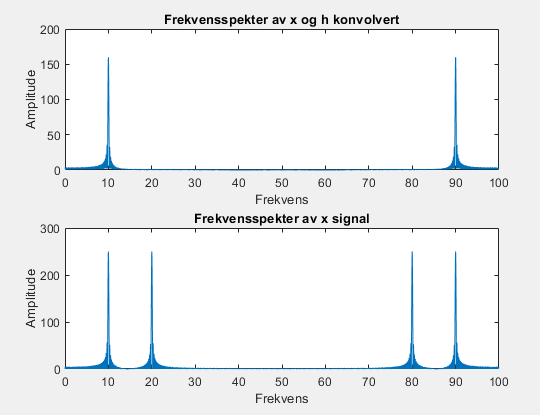
\includegraphics[scale=0.9]{1c_xh.png}
\caption{Plott av frekvensspekteret til x signalet og signalet konvolvert med filteret. Frekvens på x-aksen og amplitude på y-aksen. }
\end{figure}

\begin{figure}[H]
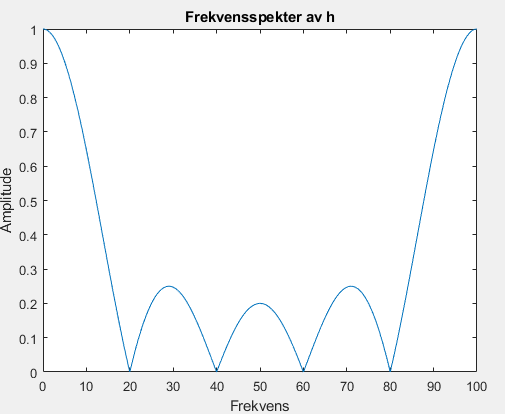
\includegraphics[scale=0.9]{1c_hfrek.png}
\caption{Plott av frekvensspekteret til filterett. Frekvens på x-aksen og amplitude på y-aksen.}
\end{figure}

Vi ser at vi får topper ved 10Hz og 90Hz på det første plott. Dette er bare en speiling, så vi ser bare på første halvpart av figurene for frekvensspekterene. Vi har to frekvenser i x-signalet, 10Hz og 20Hz. Frekvensspekteret for det konvolverte signalet har bare 10Hz, dette betyr altså at filteret har filtrert ut 20Hz fra signalet vårt, og amplituden har også blitt mindre. I frekvensspekteret til h ser vi at amplituden er 0 ved 20Hz og 40Hz, dette kan være grunnen til at det filtrerer ut 20Hz når vi konvolverer det med signalet.

Oppgave 2)
\begin{figure}[H]
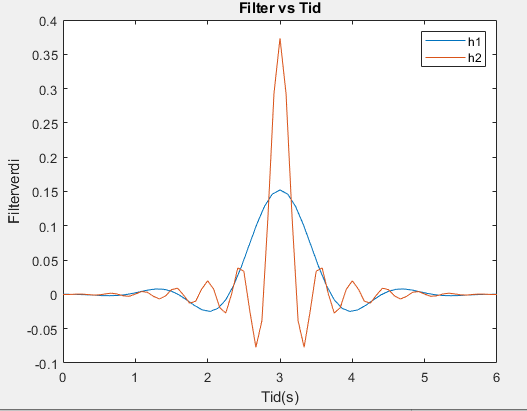
\includegraphics[scale=0.9]{2a_firtid.png}
\caption{Plott av filtrene med hensyn på tid. Filterverdi/amplitude på y aksen og tid på x aksen.}
\end{figure}

\begin{figure}[H]
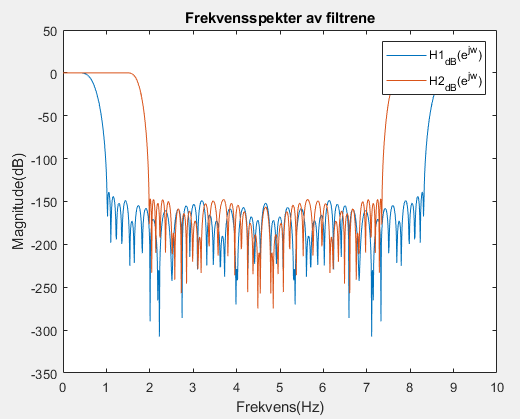
\includegraphics[scale=0.9]{2a_firfrek.png}
\caption{Plott av frekvensspekteret til de to filterene. Frekvens i dB på x-aksen og amplitude på y-aksen.}
\end{figure}

Når vi ser på frekvensspektrene til de to filtrene ser vi at de er nesten identiske. Men vi ser at h2 er 0 lengere enn h1. --Skriv mer--
\end{document} 